\section{Pretraživanje penjačkih lokacija, sektora, penjačkih lokacija i korisnika}

Kako bi korisnici mogli brzo pronaći informacije, aplikacija omogućuje pretraživanje penjačkih lokacija, sektora, penjačkih smjerova i korisnika. Pristupom zaslonu za pretraživanje ili na web aplikaciji klikom na traku za pretraživanje u navigacijskoj traci, korisniku se prikazuje traka za unos teksta te, inicijalno, popis nedavno pregledanih stavki, što omogućuje brz povratak na prethodno pregledane elemente (slika~\ref{fig:pretrazivanje_sidebyside}).

\begin{figure}[H]
    \centering
    \begin{subfigure}[b]{0.35\textwidth}
        \centering
        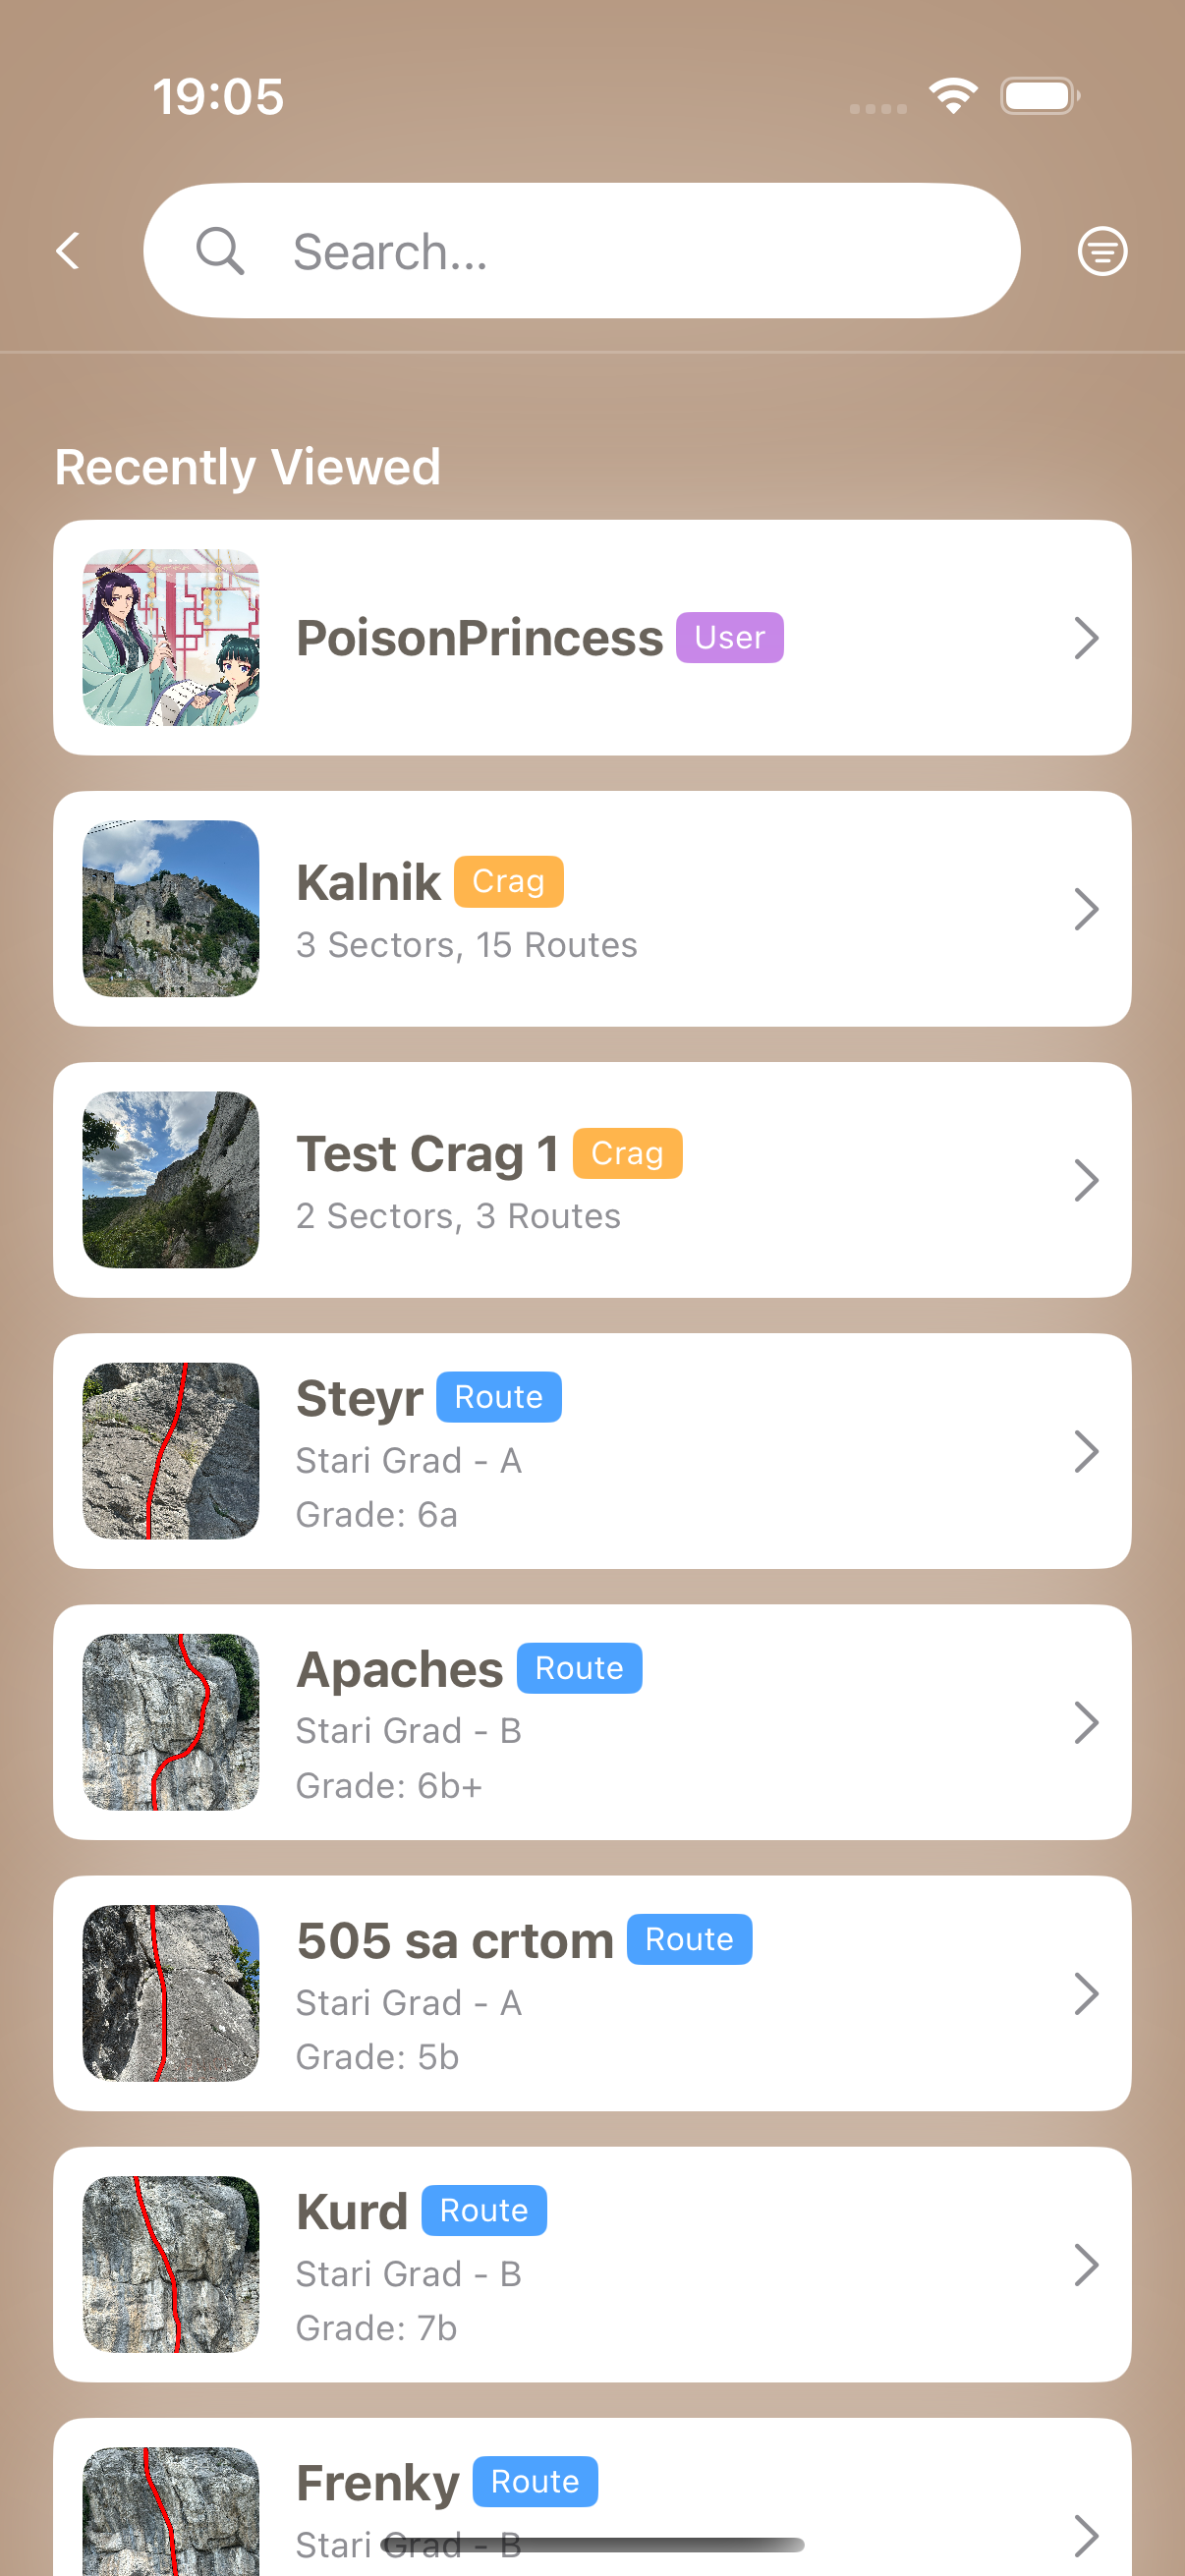
\includegraphics[width=\textwidth]{images/implementacija/search_default.png}
        \caption{Mobilna aplikacija}
        \label{fig:pretrazivanje_default}
    \end{subfigure}
    \hfill
    \begin{subfigure}[b]{0.6\textwidth}
        \centering
        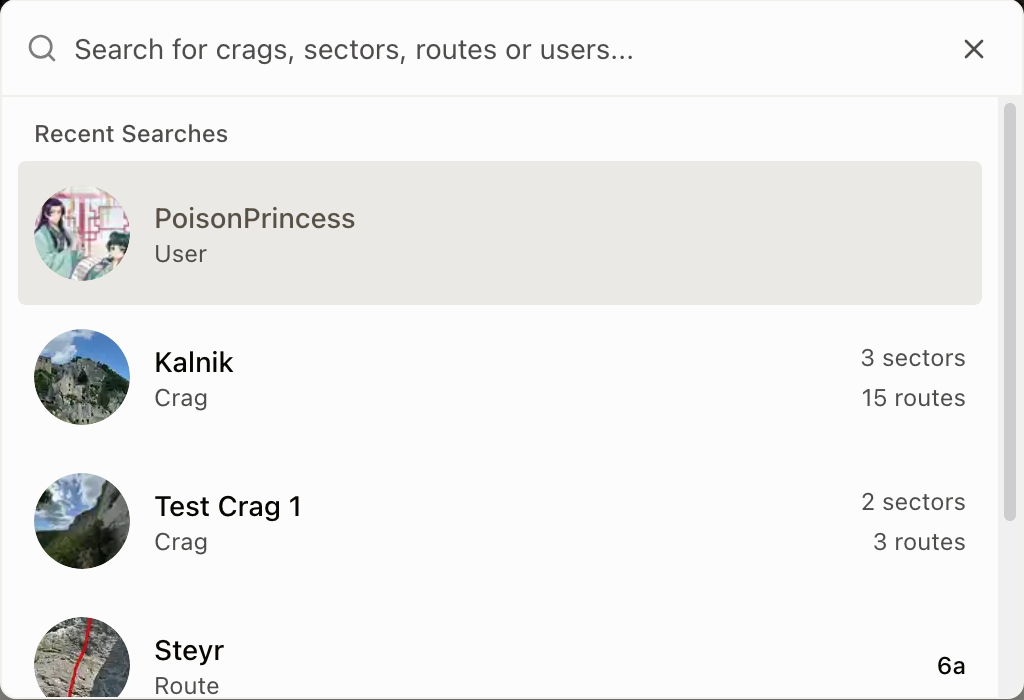
\includegraphics[width=\textwidth]{images/implementacija/web/search_default.png}
        \caption{Web aplikacija}
        \label{fig:pretrazivanje_searching}
    \end{subfigure}
    \caption{Inicijalno stanje pretraživanja - prikaz nedavno pregledanih stavki}
    \label{fig:pretrazivanje_sidebyside}
\end{figure}

Sustav pretraživanja je dinamičan i reagira na korisnikov unos. Upisivanjem pojma u traku za pretraživanje, aplikacija filtrira popis dostupnih penjačkih lokacija, sektora, penjačkih smjerova i korisnika te prikazuje relevantne rezultate iz više kategorija istovremeno (slika~\ref{fig:pretrazivanje_side_by_side}). 

\begin{figure}[H]
    \centering
    \begin{subfigure}[b]{0.35\textwidth}
        \centering
        
\includegraphics[width=\textwidth]{images/implementacija/search_searching.png}
        \caption{Mobilna aplikacija}
        \label{fig:pretrazivanje_web_1}
    \end{subfigure}
    \hfill
    \begin{subfigure}[b]{0.6\textwidth}
        \centering
        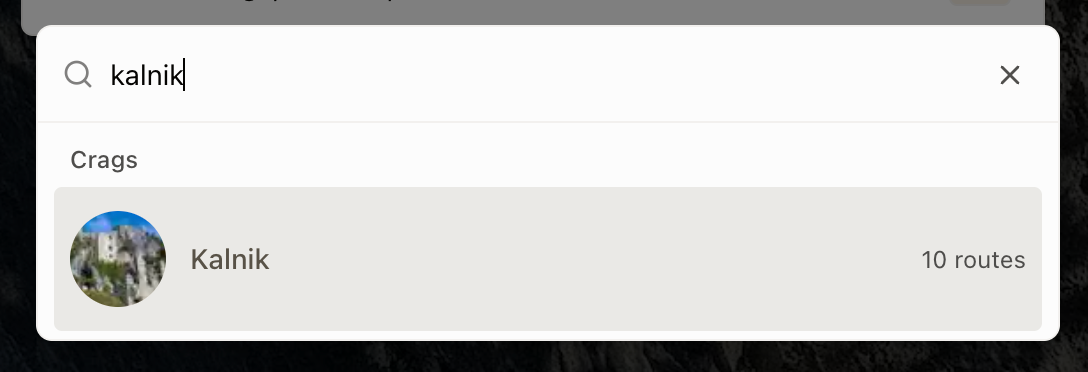
\includegraphics[width=\textwidth]{images/implementacija/web/search_searching.png}
        \caption{Web aplikacija}
        \label{fig:pretrazivanje_web_2}
    \end{subfigure}
    \caption{Funkcionalnost pretraživanja}
    \label{fig:pretrazivanje_side_by_side}
\end{figure}

Svaki rezultat pretrage prikazan je u obliku pregleda kartica koje sadrže informacije poput naziva i tipa sadržaja, te dodatne podatke ovisno o tipu sadržaja. Penjačke lokacije sadrže broj sektora i penjačkih smjerova, sektori broj penjačkih smjerova, a korisnici broj penjačkih smjerova koje su popeli. Odabirom bilo kojeg rezultata, korisnik se preusmjerava na odgovarajući detaljni prikaz. 

